\section{Les objectifs et méthodes du Machine learning}

Le choix de la méthode d'apprentissage dépend en grande partie de l'objectif
poursuivi.

\subsection{Les objectifs du machine learning}

Le machine learning poursuit plusieurs objectifs qui selon le cas peut être
 \subsubsection{Une classification}
Les modèles de classification prédisent des valeurs discrètes. Ils formulent, 
par exemple, des prédictions qui répondent à des questions telles que les suivantes:
\begin{itemize}
  \item Un e-mail donné est-il considéré comme du spam ou non?
  \item Cette image représente-t-elle un chien, un chat ou un hamster?
  \item Un dossier donné est-il conforme ou pas?
\end{itemize}

La classification est un processus en deux étapes, une étape 
d’apprentissage et une étape de prédiction, dans l’apprentissage machine.
Dans l’étape d’apprentissage, un modèle est développé à partir d’un 
ensemble de données préalablement étiquettés. Dans la phase de prédiction,
le modèle développé dans la phase précédente est utilisé pour prédire les 
étiquettes de nouvelles données.

\subsubsection{Une regression}
Les modèles de régression prédisent des valeurs continues. Ils formulent,
par exemple, des prédictions qui répondent à des questions telles que :
\begin{itemize}
  \item Quel est la valeur d'un logement au Burkina Faso ?
  \item Quel est la probabilité qu'un utilisateur clique sur cette annonce?
\end{itemize}

\subsubsection{Le clustering}
Le clustering est le regroupement d'exemples en classes d'objets similaires.
La différence entre clustering et classification est que les exemples sont
étiquetés dans une classification alors que dans le clustering, il ne le sont
pas.(Voir Figure \ref{fig:clustering})


\begin{figure}[h!]
  \begin{center}
    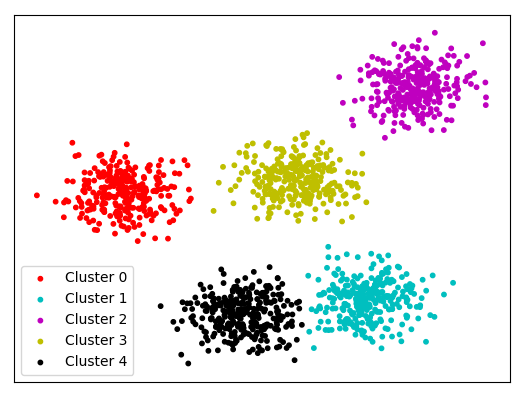
\includegraphics[width=14cm]{images/clustering.png}
      \caption{Clustering des données.\label{fig:clustering}}
  \end{center}
\end{figure}

Le but des algorithmes de clustering est de donner un sens aux données et
d'extraire de la valeur à partir de grandes quantités de données structurées ou
non-structurées. Ces algorithmes vont permettre de séparer les données en
fonction de leurs propriétés ou fonctionnalités et de les regrouper dans
différents clusters en fonction de leurs similitudes.




\subsection{Les méthodes d'aprentissage}
Les méthodes d'apprentissage automatique les
plus largement adoptées sont l'apprentissage supervisé et l'apprentissage
non-supervisé. Explorons donc ces méthodes plus en détail.

\subsubsection{L'apprentissage supervisé}
Le but de cette méthode est de permettre à l'algorithme  de découvrir 
l'étiquette réelle d'un exemple à partir des étiquettes apprises pendant la
phase d'entrainement, pour trouver des erreurs et modifier le modèle en 
conséquence. L'apprentissage supervisé utilise pour l'entrainement de son modèle,
des exemples étiquettés.

\subsubsection{L'apprentissage non-supervisé}
L’apprentissage non supervisé consiste à apprendre à classer sans supervision; les
exemples fournis sont non-étiquettés. L'objectif ici  est de réunir les 
exemples selon des critères prédéfinis par les équipes en charge du projet.En effet,
l’apprentissage non supervisé permet de regrouper des éléments non-classés dans 
différents groupes selon leurs caractéristiques.
